\begin{XeClass}{FSInputStream}
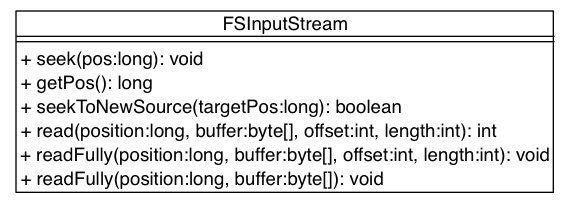
\includegraphics[width=\textwidth]{cdig/FSInputStream.png}
     
 FSInputStream 是一个抽象类,继承了基本的\emph{java.io.InputStream}, 并且提供了
 随机文件读写(Random Access File)的能力。

    \begin{XeMethod}{\XePublic \\ \XeAbstract}{void}{seek}
         
 Seek方法将当前读取位置移动到\emph{pos},读取位置都是相对
 于文件的开头,下一次read()调用将会从\emph{pos}处开始
 读取。该方法不能将读取位置设置到超出文件长度的位置。

    \end{XeMethod}

    \begin{XeMethod}{\XePublic \\ \XeAbstract}{long}{getPos}
         
 返回当前的读取位置,该读取位置相对于文件开始处。

    \end{XeMethod}

    \begin{XeMethod}{\XePublic \\ \XeAbstract}{boolean}{seekToNewSource}
         
 将输入源切换到一个新的输入源,并且将读取位置移动到\emph{pos}。
 此方法在FTP、S3、Local等文件系统上均无实现(直接返回false),现有
 的唯一实现在\emph{org.apache.hadoop.hdfs.DFSInputStream.seekToNewSource(long targetPos)},其功能是在当前读取的Block失效时,切换到新的Block,并且移动读取位置,操作成
 功时返回true。

    \end{XeMethod}

    \begin{XeMethod}{\XePublic}{int}{read}
         
 该方法可以从指定的文件位置处,往buffer指定的字节数组的offset位置读入length
 个字节,并且可以恢复文件读取位置到读取之前的状态,并且该方法是线程安全的。

    \end{XeMethod}

    \begin{XeMethod}{\XePublic}{void}{readFully}
         
 该方法与 \emph{FSInputStream.read(long,byte[],int,int)}类似,
 但是read方法允许读取到的字节数小于length,而readFully方法一定读取到length
 个字节,除非出现EOF或者 \emph{java.io.IOException}

    \end{XeMethod}

    \begin{XeMethod}{\XePublic}{void}{readFully}
         
 \emph{FSInputStream.readFully(long,byte[],int,int)}的另一个版本,
 即从buffer的开始处放入buffer长度个字节。

    \end{XeMethod}

\end{XeClass}
